\documentclass[11pt]{article}
\usepackage{graphicx}
\usepackage[utf8]{inputenc}
\usepackage{enumerate}
\usepackage{multirow,tabularx}
\usepackage{caption}
\usepackage{subfigure}
\usepackage[T1]{fontenc}
\usepackage{mathptmx}
\usepackage[a4paper, left=2cm, right=2cm, top=2.5cm, bottom=2.5cm, headsep=1.2cm]{geometry} 
\usepackage[rightcaption]{sidecap}
\usepackage{float}
\usepackage{pgfplots}
\pgfplotsset{compat=1.14}
\begin{document}

\begin{titlepage}

	\begin{center}

    


	\huge{\textsc{Metody Komputerowe w Spalaniu}} \\
[50mm]

    \LARGE{\textbf{Hydrogen-air mixture ZND detonation.
}} \\
	[50mm]
	\Large{Norbert Czarnota}\\
    \Large{271292}\\
    [25mm]
    \large{Aerospace Engineering}\\
    [80mm]
    \large{Warsaw, 28.06.2017}\\
    \end{center}
    
\end{titlepage}

\newpage



\section{Purpose of the project}
The purpose of the project was to simulate the ZND detonation and compare the results with the experimental data using SDToolbox for Matlab. The calculations were performed for different equivalence ratio (from 0,7 to 1,78).

\section{Mathematical model}
The ZND detonation model is a one-dimensional model for the process of detonation of an explosive. It was proposed during World War II independently by Y. B. Zel'dovich, John von Neumann, and Werner Döring, hence the name.
This model admits finite-rate chemical reactions and thus the process of detonation consists of the following stages. First, an infinitely thin shock wave compresses the explosive to a high pressure called the von Neumann spike. At the von Neumann spike point the explosive still remains unreacted. The spike marks the onset of the zone of exothermic chemical reaction, which finishes at the Chapman-Jouguet state. After that, the detonation products expand backward. In the reference frame in which the shock is stationary, the flow following the shock is subsonic. Because of this, energy release behind the shock is able to be transported acoustically to the shock for its support. For a self-propagating detonation, the shock relaxes to a speed given by the Chapman–Jouguet condition, which induces the material at the end of the reaction zone to have a locally sonic speed in the reference frame in which the shock is stationary. In effect, all of the chemical energy is harnessed to propagate the shock wave forward.
However, in the 1960s, experiments revealed that gas-phase detonations were most often characterized by unsteady, three-dimensional structures, which can only in an averaged sense be predicted by one-dimensional steady theories. Indeed, such waves are quenched as their structure is destroyed. The Wood-Kirkwood detonation theory can correct for some of these limitations. 


\section{Results and plots}

\begin{figure} [H]
	\begin{center}
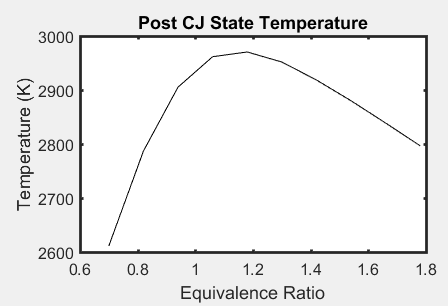
\includegraphics[height=0.5\textwidth]{P1}
    \end{center}
\end{figure}

\begin{figure} [H]
	\begin{center}
    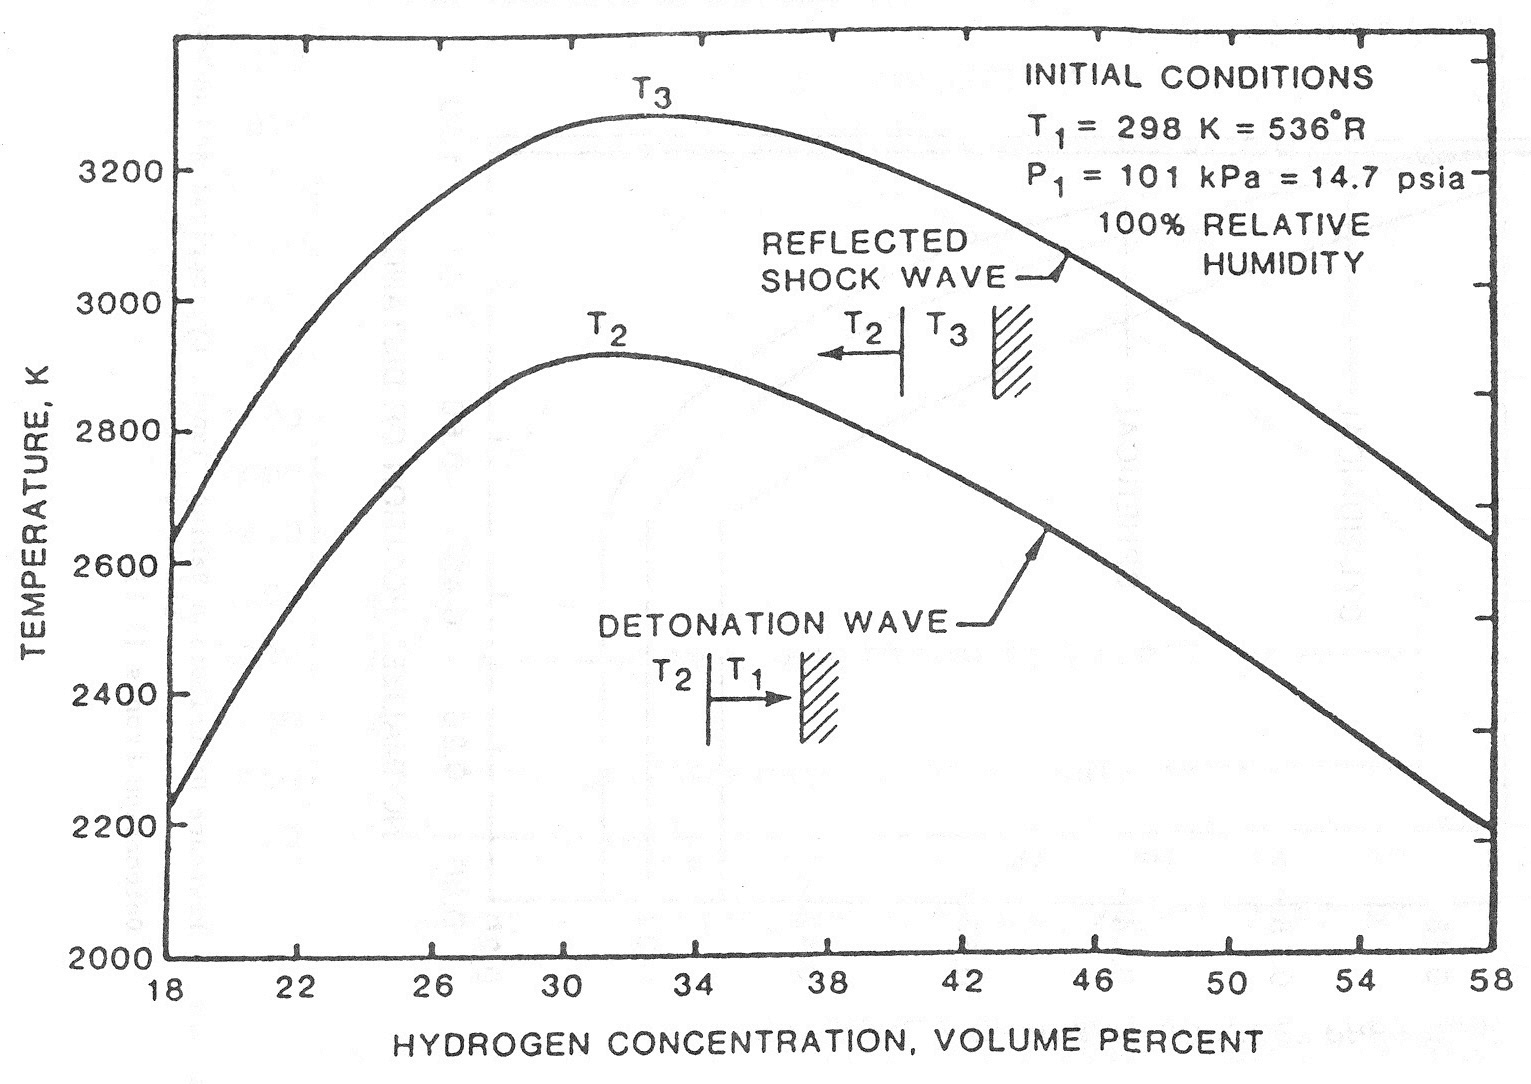
\includegraphics[height=0.5\textwidth]{E1}
    \end{center}
\end{figure}
The first plot get from calculations compared to experimental data (second plot). The difference in max temperature =100 K. The shape of the first plot is similar to experiment alongside with the concentration.
\begin{figure} [H]
	\begin{center}
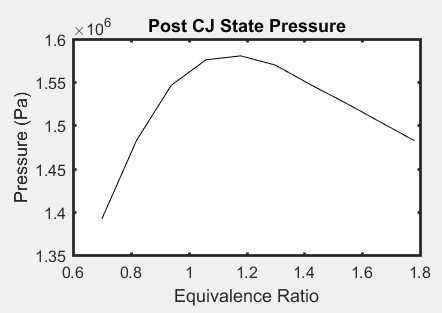
\includegraphics[height=0.5\textwidth]{P2}
    \end{center}
\end{figure}
Values for pressure and shape of the plot are comparable and similar to experimental data.
\begin{figure} [H]
	\begin{center}
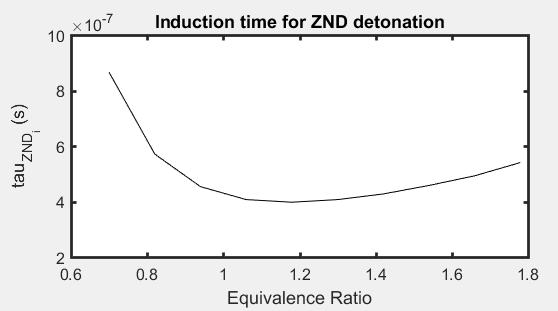
\includegraphics[height=0.5\textwidth]{P3}
    \end{center}
\end{figure}

\begin{figure} [H]
	\begin{center}
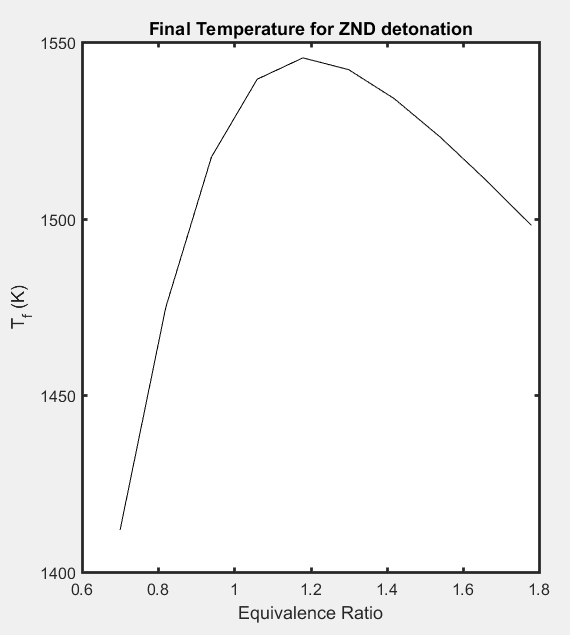
\includegraphics[height=0.5\textwidth]{P4}
    \end{center}
\end{figure}




\section{References}
\begin{enumerate}
	\item{https://en.wikipedia.org/wiki/ZND$detonation$model}
    \item{http://gasturbinespower.asmedigitalcollection.asme.org/article.aspx?articleid=1661514}
    \item{http://www.hysafe.net/wiki/BRHS/ChemicalPropertiesOfHydrogenf}
     \item{http://shepherd.caltech.edu/EDL/public/cantera/html/SD$Toolbox/$MatlabInstall}
\end{enumerate}










\end{document}